\documentclass[tikz, border=10pt]{standalone}
\usepackage{tikz}
\usetikzlibrary{calc}

\begin{document}
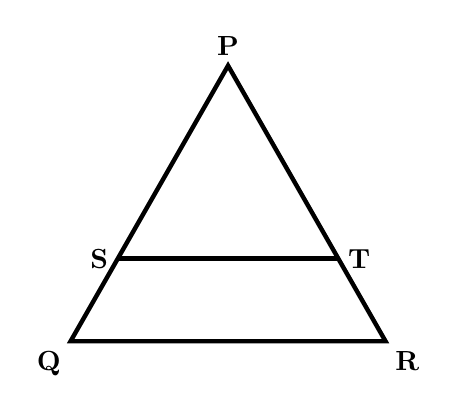
\begin{tikzpicture}

% Define vertices of the main triangle
\coordinate (P) at (2, 3.5);
\coordinate (Q) at (0, 0);
\coordinate (R) at (4, 0);

% Define points S and T on the sides (parallel to QR)
% S on PQ, T on PR (about 40% from bottom)
\coordinate (S) at ($(Q)!0.3!(P)$);
\coordinate (T) at ($(R)!0.3!(P)$);

% Draw the main triangle PQR
\draw[ultra thick] (P) -- (Q) -- (R) -- cycle;

% Draw the parallel line ST
\draw[ultra thick] (S) -- (T);

% Labels
\node[above] at (P) {\textbf{P}};
\node[below left] at (Q) {\textbf{Q}};
\node[below right] at (R) {\textbf{R}};
\node[left] at (S) {\textbf{S}};
\node[right] at (T) {\textbf{T}};

\end{tikzpicture}
\end{document}